\documentclass[12pt]{article}
\usepackage{chemfig}
\usepackage{graphicx}
\usepackage{gensymb}
\usepackage[version=4]{mhchem}
\usepackage{polyglossia}
\usepackage{fontspec}
\usepackage{titlesec}
\usepackage{lettrine}
\usepackage{epigraph, varwidth}
\setlength{\epigraphwidth}{0.8\textwidth}
% sectioning used with \paragraph{at subsubsubsection}
\setcounter{secnumdepth}{4}
\titleformat{\paragraph}
{\normalfont\normalsize\bfseries}{\theparagraph}{1em}{}
\titlespacing*{\paragraph}
{0pt}{3.25ex plus 1ex minus .2ex}{1.5ex plus .2ex}
% sectioning
\setdefaultlanguage{english}
\setotherlanguages{marathi}
\newfontfamily\marathifont[Mapping=velthuis-sanskrit,Script=Devanagari,Language=Marathi]{Shobhika}
\usepackage{hyperref}
\hypersetup{
    backref,
    colorlinks=true,
    filecolor=magenta,
    linkcolor=blue,
    urlcolor=cyan,
}
\urlstyle{same}
\begin{document}
\title{Self-study Notes on OpenStax AP Biology Books and Other Resources}
\author{Kedar Mhaswade}
\date{2020-21}
\maketitle
\def\dev{\edef~{\string~}\textmarathi}
\section{The Cell}
\subsection{Cell Structure}
\subsection{Structure and Function of Plasma Membranes}
\subsection{Metabolism}
\subsubsection{ATP: Adenosine Tri-Phospate}
\begin{itemize}
    \item Even exergonic reactions (those that \textit{release} energy) require a small amount of
        \textit{activation energy} to proceed.
    \item Products of endergonic reactions (those that \textit{require} energy input) have
        more energy than that of their reactants. Where does the cell provide this energy from?
    \item ATP is the molecule that provides the energy required for the endergonic reactions 
        as well as the small activation energy required for the exergonic reactions.
    \item ATP is a \textit{relatively} simple molecule: C\textsubscript{10}H\textsubscript{16}N\textsubscript{5}O\textsubscript{13}P\textsubscript{3} %$C_{10}H_{16}N_{5}O_{13}P_{3}$
        \begin{itemize}
            \item It has adenosine bound to three phosphate groups that are named alpha- (closest to ribose), beta-, and gamma-phosphate (farthest from ribose).
            \item Adenosine is a \textit{nucleoside}---a compound commonly found in DNA or RNA, consisting of a purine or pyrimidine base linked to a sugar.
        \end{itemize}
    \item ATP \textit{hydrolyzes} to ADP (Adenosine Di-Phosphate) and inorganic phosphate. Regeneration of ATP requires energy to be supplied. Thus, hydrolysis of ATP is reversible: \\
        \schemestart ATP + H\textsubscript{2}O\arrow{<=>}ADP + P\textsubscript{i} + free energy\schemestop\par
    \item Cellular conditions differ from standard conditions. In cellular conditions, the $\Delta G$ (change in Gibbs free energy) of ATP's hydrolysis is -57 kJ/mol = -14 kcal/mol.
\end{itemize}

\subsection{Photosynthesis}
\emph{Many organisms} access stored energy by \emph{eating} or \emph{ingesting (consuming)} other organisms: \textmarathi{jiivo jiivasya jiivanam|}. All of this energy can be traced back to photosynthesis.
\subsubsection{Overview}
Photosynthesis is the \emph{only} biological process that can capture the energy in sunlight and convert it into the energy stored in the covalent bonds of sugar molecules. Additionally, it acts as a source of oxygen necessary for \emph{many} living organisms.

\emph{Photoautotrophs} (organisms that use light to synthesize their own food) such as plants, algae(\textmarathi{\dev aljii}), and cyanobacteria are the only ones that can perform photosynthesis.

\emph{Chemoautotrophs} (organisms that use energy stored in inorganic molecules, and not sunlight, to synthesize their own food) found in deep sea represent another class of \emph{autotrophs}.

Animals, fungi, and most other bacteria are termed \emph{Heterotrophs} because they have to rely on the sugars produced by Photoautotrophs.

\paragraph{Main Structures and Summary}
Photosynthesis is a multi-step process that requires
\begin{enumerate}
    \item Specific wavelengths of visible sunlight and
    \item Carbon dioxide (low in energy) and water as substrates.
\end{enumerate}
It 
\begin{enumerate}
    \item Releases oxygen and
    \item Produces glyceraldehyde 3-phosphate (G3P) which can be synthesized into different sugar molecules (G3P has three carbon atoms; two G3P molecules form one glucose molecule). G3P is formed when one CH2OH from glycerol is replaced in an aldehyde and then a hydrogen is replaced by phosphate (H2PO4-).
\end{enumerate}
\begin{figure}[ht!]
    \centering
    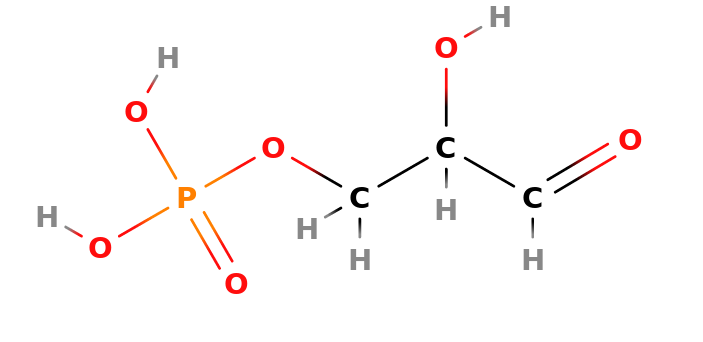
\includegraphics[width=0.8\linewidth]{g3p.png}
    \caption{Glyceraldehyde-3 phosphate}
    \label{fig: g3p}
\end{figure}

The effective chemical equation of photosynthesis is:

\ce{6CO2 + 6H2O ->[Sunlight] C6H12O6 + 6O2}

But note that there are several steps involved in this transformation.

\paragraph{Basic Photosynthetic Structures}
\begin{enumerate}
    \item In plants, it generally takes place in \emph{leaves} which have several layers of cells. The layer for photosynthesis is called \emph{mesophyll} (Greek: \emph{meso}: in the middle, \emph{-phyll}: leaf or pigment)
    \item The gas exchange takes place through \emph{stomata} (Greek: \emph{stoma}: mouth or opening)
\end{enumerate}

\subsection{Cell Communication}
\subsubsection{Signaling Molecules and Cellular Receptors}
\paragraph{Introduction}
In order to respond properly to external stimuli, cells have developed \emph{sophisticated} mechanisms of communication that can
\begin{enumerate}
    \item receive a \emph{message},
    \item transfer the information across the plasma membrane, and
    \item produce changes in the cell as a response
\end{enumerate}
Both single-celled (yes, single-celled) and multicellular organisms communicate with each other at a cellular level and across the organisms.

Communication within a cell is called the \emph{intracellular} communication, whereas the communication between two or more cells is called the \emph{intercellular} communication.

The small, usually volatile, and soluble signaling molecules that \emph{bind} to another specific molecule (and deliver a signal in the process) are called \emph{ligands}.

Ligands bind or interact with proteins called the \emph{receptor proteins} in the \emph{target cells} (the cells that would be affected by the ``signals''). Specific ligands bind with specific receptors. 

\subsection{Cell Reproduction}
\subsubsection{Introduction}
\textbf{A human, like every sexually reproducing organism, begins life as a fertilized egg (embryo) or zygote}. All multicellular organisms use cell division (even after they are fully grown) for growth and maintenance and repair of cells and tissues. Cell division is \emph{regulated closely}. Unicellular organisms also use cell division for their reproduction. 

Not all cells in the human body can reproduce \emph{to repair tissues}. Most nerve cells, for example, are not capable of regeneration. This means that people who have damaged their nerve cells or nervous system are often left paralyzed\footnote{This may change because of research}.
\subsubsection{Cell Division}
The cell cycle is an orderly sequence of events. It describes the stages of a cell's life from the division of a single parent cell to the production of two new genetically identical daughter cells.
\paragraph{Genomic DNA}
A cell's DNA, packaged as a double-stranded DNA molecule, is called its \emph{genome}. 

\lettrine[lines=2]{I}{n prokaryotes}, the genome is composed of a single DNA molecule. It's found in an area called \emph{nucleoid}. Sometimes, smaller loops of DNA called \emph{plasmids} are also present. Prokaryotes exchange plasmids with other prokaryotes. \emph{Antibiotic resistance} may be developed in a bacteria colony as a result of plasmid exchange between a resistant donor and recipient cells.

\lettrine[lines=2]{I}{n eukaryotes}, the genome is composed of several \emph{double stranded} linear DNA molecules. Each species has a \emph{characteristic number} of chromosomes. Human somatic (body) cells have 46 chromosomes, whereas human gametes (sperm or egg cells) have 23 chromosomes each.

\textbf{Matched pairs of chromosomes in a diploid organism are called \underline{homologous chromosomes}}. Each copy of a homologous chromosome originates in a different parent. The individual homologous chromosome therefore is not identical to its copy. \textbf{Regions of chromosome are identified as genes}. Genes are the \emph{functional units} of chromosome and they determine the phenotypical (externally visible) characteristics of an individual by \emph{encoding specific proteins}. 

A location on a chromosome is called \textbf{locus} and a gene is said to be located at some locus. Since there are population variations, two different humans are more likely to have variations in the genes. Although we do not have the DNA sequence of each human, there are statistical models that determine the form or version of each gene. \textbf{Each form or version of a gene at a given locus is called an allele}.
\subsubsection{The Cell Cycle}
\subsubsection{Control of the Cell Cycle}
\subsubsection{Cancer and the Cell Cycle}
\subsubsection{Prokaryotic Cell Division}

\section{Unit 3: Genetics}
\subsection{Meiosis and Sexual Reproduction}
\subsection{Mendel's Experiments and Heredity}

\subsubsection{Mendel's Experiments and the Laws of Probability}
Johann Gregor Mendel conducted experiments to demonstrate the existence of genes long before the term was coined. His experiments are an exemplary lesson in the ``design and execution of scientific experiments''. Mendel is regarded as the father of modern genetics.

\subsubsection{Extra: Mendel's Experiments (Refers to Various Resources)}
Mendel wanted to investigate if there was a \emph{general law} for the formation and development of \emph{hybrids}, something he noted had not been previously formulated \cite{mendel-fisher}: 
\epigraph
{
    Those who survey the work done in this department will arrive at the conviction that among all the numerous experiments made, \emph{not one has been carried out to such an extent and in such a way as to make it possible to determine the number of different forms under which the offspring of hybrids appear}, or to arrange these forms with certainty according to their separate generations, or definitely to ascertain their statistical relations.
}
{
    ---\textit{Johann Gregor Mendel \cite{mendel-fisher}}
}

Mendel and his colleagues carried out their experiments for nearly a decade (1856-1865). Mendel required \cite{mendel-fisher} that the experimental plant must
\begin{enumerate}
    \item possess constant differentiating factors
    \item be capable, during flowering, of protecting from the influence of \emph{foreign pollen}
\end{enumerate}

After careful analysis of various options, Mendel chose ``garden pea'' (\emph{Pisum Sativum L.}) to experiment with. He decided to experiment with the garden pea and examine following traits:
\begin{enumerate}
    \item Seed shape: Round or Wrinkled (a \emph{seed\footnote{A characteristic that can be ascertained by simply analyzing the seed}} characterestic)
    \item Cotyledon (the first leaves that sprout out of the seed upon germination) color: Yellow or Green (a seed characteristic)
    \item Seed-coat color: Colored or White (a \emph{plant\footnote{A characteristic that can only be ascertained by waiting for a plant to grow from the seed} characteristic})
    \item Pod shape: Inflated or Constricted (a plant characteristic)
    \item Pod color: Green or Yellow (a plant characteristic)
    \item Flower position: Axial (along the stem) or Terminal (at the end of the stem) (a plant characteristic)
    \item Stem length: Long (6--7 feet) or Short (less than a foot) (a plant characteristic)
\end{enumerate}

An interesting and somewhat philosophical question arises: ``Chicken first or egg first?'' Mendel tried to answer it from what he had available: Generations of true-bred plants. 

There is a lot of terminology here and we need to understand just what the \emph{key terms} mean before proceeding. We should also put ourselves into Mendel's shoes and try to reason the way he did. Explaining what Mendel did using the modern Genetics terms is likely to be disappointing. For example, we shouldn't be using a term like \emph{homozygous} because Mendel didn't even know what that term meant. Of course, at some point we should reconcile all of this in terms of contemporary knowledge. 

Here are the key terms in the order of their dependence (i.e. a term appearing later in the list will depend on the terms appearing before):
\begin{enumerate}
    \item \textbf{Characteristic}:
    \item \textbf{True-bred}: This is an adjective, typically applied to a plant or species. It also applies to a Characteristic.
\end{enumerate}

\subsubsection{Characteristics and Traits}
\subsubsection{Laws of Inheritance}

\subsection{Modern Understandings of Inheritance}
\subsection{DNA Structure and Function}
\subsection{Genes and Proteins}
\subsection{Gene Regulation}
\subsection{Biotechnology and Genomics}

\section{Unit 4: Evolution}
\subsection{Evolution and Origin of Species}
\subsection{The Evolution of Populations}
\subsection{Phylogenies and the History of Life}

\section{Unit 5: Viruses}

\begin{thebibliography}{00}
    \bibitem{mendel-fisher} Allan Franklin, A. W. F. Edwards, Daniel J. Fairbanks, Daniel L. Hartl. Ending the Fisher-Mendel Controversy. University of Pittsburgh Press, 2008. Page 2.
\end{thebibliography}
\end{document}
